%!TEX root = ../report.tex
\documentclass[report.tex]{subfiles}
\begin{document}
    \chapter{Evaluation and Results}

    \section{Experiment Description}

    Describe the experiments/evaluation you are performing to analyse your method.

    \section{Experimental Setup}

    Describe your experimental setup in detail.


    % For SAF FCOS
        %  Use this in experiment section
        % - Training Implementation

        %     - It uses SGD with momentum and weight decay, and train for 12 epochs. The official implementation uses batch size of 16 with LR of 0.01 but due to computational limitations, we have used LR 0.001 with reduced batch size 8. It uses warmup scheme for the first few iterations of training.

        %     The training process involves Stochastic Gradient Descent (SGD) with momentum and weight decay, spanning 12 epochs. While the official implementation opts for a batch size of 16 and a learning rate of 0.01, computational constraints led us to use a reduced batch size of 8 and a learning rate of 0.001. A warmup scheme is employed during the initial iterations of training.

        % % TODO: MOVE this section to experiment setup section
        % % \textbf{Dataset split}: 
        % \paragraph*{Dataset Split}
        % The method limits its focus on detecting vehicular obstacles such as — bicycles, cars, motorcycles, buses, trailer, and trucks—collectively categorized as 'vehicles' for simplified classification. Pedestrians are excluded due to radar detection limitations in the nuScenes dataset. Emphasis is placed on front camera data from nuScenes, with the dataset split detailed in Figure \ref{fig:saffcos_data_split}.

        % \begin{figure}[h!]
        %     \centering
        %     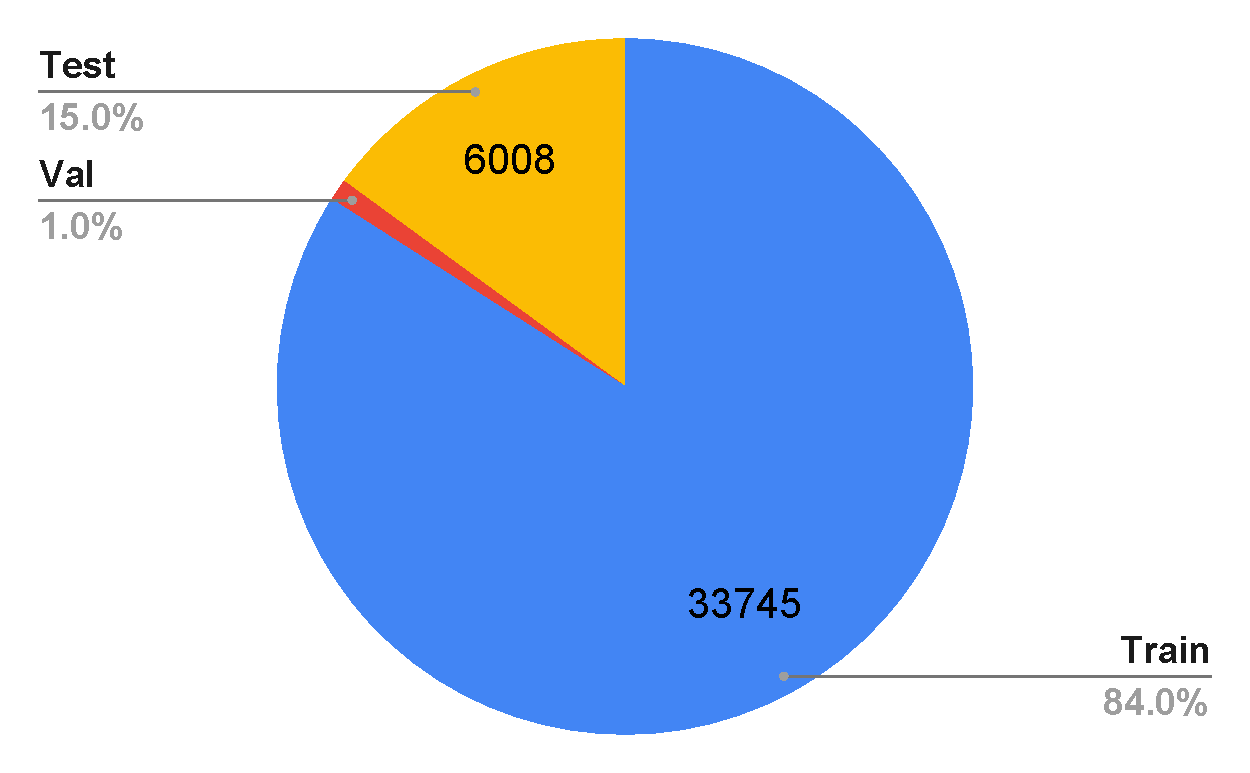
\includegraphics[width=0.5\textwidth]{images/methods/saf_fcos/data_split.pdf}
        %     \caption{Data split of nuScenes dataset. Total samples: 40157. Note: this is a custom dataset split chosen by the authors.}
        %     \label{fig:saffcos_data_split}
        % \end{figure}

    \section{Results}

    Describe the results of your experiments in detail.

\end{document}
